
\section{Tabelas}

A água pode se encontrar em mudança de fase, por exemplo, na vaporização estão presentes duas fases, a fase líquida e a fase gasosa:

\begin{eqnarray}
    V = V_{liq} + V_{vap}\\
    v = \frac{V_{liq} + V_{vap}}{m}
\end{eqnarray}

onde $V_{liq} = m_{liq} v_f$ e $V_{vap} = m_{vap} v_g$, pelo que:

\begin{equation}
    v = \frac{m_{liq}}{m} v_f + \frac{m_{vap}}{m} v_g
\end{equation}

Definindo $x = \frac{m_{vap}}{m}$, como o título da água, temos $\frac{m_{liq}}{m} = 1 - x$ e podemos escrever:

\begin{equation}
    v = (1-x) v_f + x v_g = v_f + x(v_g - v_f)
\end{equation}

E, portanto,

\begin{equation}
    x = \frac{v-v_f}{v_g-v_f}
\end{equation}

\begin{figure}[H]
    \centering
    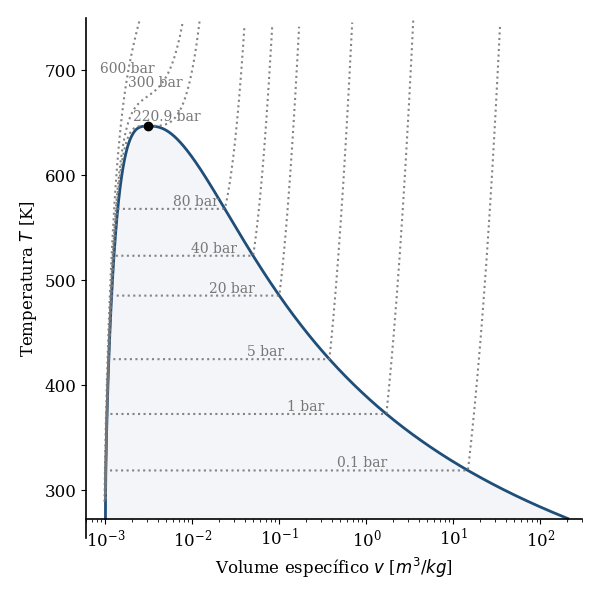
\includegraphics[width=0.4\linewidth]{graphs/water-dome-Tv-critical.png}
    \caption{Diagrama T-v da água}
    \label{fig:water-dome-Tv}
\end{figure}

É possível verificar que para uma pressão de $1.01325~\text{bar} = 1~\text{atm}$, a temperatura de saturação é $100~\text{\textdegree C} = 373.15~\text{K}$ -- i.e. a temperatura à qual ocorre a vaporização da água em condições de pressão atmosférica.

O ponto crítico da água ocorre a uma pressão de $p = 22.09~\text{MPa} = 220.9~\text{bar}$ e temperatura de $T = 647.096~\text{K}$.

Nas curvas de pressão constante -- \textbf{isobáricas} --, observa-se que, para pressões acima da pressão crítica, a temperatura aumenta continuadamente com o aumento do volume específico (os termos líquido e vapor perdem significado para estas pressões). 

Por outro lado, para pressões abaixo da pressão crítica, existe uma região bifásica, onde mantendo uma pressão fixa, a temperatura permanece constante durante a vaporização, enquanto o volume específico aumenta.

\begin{figure}[H]
    \centering
    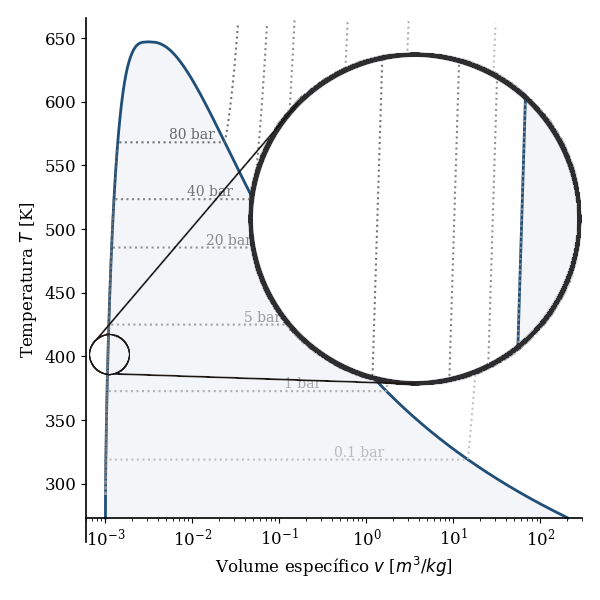
\includegraphics[width=0.4\linewidth]{graphs/water-dome-Tv-circle.png}
    \caption{Isobáricas no domo da água ampliadas}
    \label{fig:water-dome-Tv-amp}
\end{figure}

Neste gráfico consegue-se ver que para a água em líquido comprimido aproximar $u(T, p) \approx u_f(T)$, $h(T, p) \approx h_f(T)$, etc, é uma boa aproximação, já que $v \approx \text{const}$.

\begin{equation}
    u = (1-x) u_f + x u_g = u_f + x(u_g - u_f)
\end{equation}

\begin{equation}
    h = (1-x) h_f + x h_g = h_f + x(h_g - h_f)
\end{equation}

O aumento de entalpia durante a vaporização é $h_{fg} = h_g - h_f$, então: $h = h_f + x h_{fg}$.

\section{Escalas Termodinâmicas de Temperatura}

Existem duas escalas termodinâmicas de temperatura, ou seja, onde a temperatura menor é 0. Estas são a Escala de Kelvin e a Rankine.

\begin{equation}
    T(\text{\textdegree R}) = 1.8 \, T(\text{K})
\end{equation}

Por convenção internacional, as escalas de temperatura são definidas para o facilmente reproduzível ponto triplo da água - estado de equilíbrio entre vapor, gelo e água líquida. Este encontra-se a 273.16 K. O ponto de gelo da água (equilíbrio entre gelo e água saturada com ar) a 1 atm é 273.16 K até o ponto de equilíbrio de vapor e água líquida a 1 atm são 100 K.

A diferença de temperatura é igual na escala de Kelvin e na de Celsius. 

\begin{equation}
    T(\text{\textdegree C}) = T(\text{K}) - 273.15
\end{equation}

Um grau na escala de Fahrenheit tem a mesma magnitude que um grau na escala de Rankine.

\begin{equation}
    T(\text{\textdegree F}) = T(\text{\textdegree R}) - 459.67
\end{equation}

O ponto de gelo na escala de Fahrenheit encontra-se a 32 \textdegree F (0 \textdegree C) e o ponto de evaporação a 212 \textdegree F (100 \textdegree C). 180 Fahrenheit/Rankine entre os dois pontos. 
\begin{equation}
    T(\text{\textdegree F}) = 1.8 \, T(\text{\textdegree C}) + 32
\end{equation}


\section{Constante Universal dos Gases}

Define-se o volume específico por quantidade molar: $\bar{v} = M v$, onde $M$ é a massa molar e $v$ o volume específico. A sua unidade é $\text{kg}/\text{kmol}$.

Considerando um sistema êmbolo-cilindro com gás a temperatura constante, pode-se calcular o rácio $p \bar{v} / T$ para diferentes volumes (i.e., diferentes posições do êmbolo), em função da pressão. Para diferentes temperaturas, os gráficos de $p \bar{v} / T$ tendem para o mesmo valor quando a pressão se aproxima de zero.

Este comportamento sugere que, a pressões suficientemente baixas, todos os gases obedecem aproximadamente à relação:


\begin{equation}
    \lim_{p \to 0} \frac{p \bar{v}}{T} = \mathcal{R}
\end{equation}

Repetindo o processo para diferentes gases obtém-se sempre o mesmo valor, que se define como a \textbf{constante universal dos gases}:

\begin{equation}
    \mathcal{R} = 8.314~\text{kJ}/(\text{kmol}\cdot\text{K})
\end{equation}

No Shapiro, é usado para a constante universal dos gases: $\bar{R}$. 

A equação pode ser reescrita:

\begin{equation}
    \lim_{p \to 0} \frac{p \bar{v}}{\mathcal{R} T} = 1 \Longleftrightarrow \lim_{p \to 0} \frac{p \bar{v}/M}{T \mathcal{R} /M} = 1 \Longleftrightarrow \lim_{p \to 0} \frac{p v}{T \mathcal{R} / M} = 1
\end{equation}

\begin{equation}
    \lim_{p \to 0} \frac{p v}{R T} = 1
\end{equation}

onde $R$ é a constante de cada gás (nas aulas usa-se $R_0$), que é tanto maior quanto menor a massa molar $M$ do gás, cujas unidades são $\text{kJ}/\text{kg}\cdot\text{K}$ ($\text{kJ} \; \text{kg}^{-1} \; \text{K}^{-1}$). $R = \frac{\mathcal{R}}{M}$

\begin{historybox}[Lei dos Gases Ideais]
    \textbf{Boyle e a Lei dos Gases}

    Robert Boyle (1627-1691), inspirado pelos trabalhos de Torricelli e com a ajuda de Robert Hooke executou, em 1662, uma experiência que levou à formulação da Lei de Boyle. Utilizando um tubo em forma de ``J'', com mercúrio e ar aprisionado numa extremidade, Boyle mediu a variação de volume do ar em função da pressão exercida pelo mercúrio. Os dados mostravam uma relação inversa entre pressão e volume: \( pV = \text{const} \).

    Esta observação lançou as bases para a teoria cinética dos gases: ao reduzir o volume, aumenta-se a frequência de colisões moleculares com as paredes, aumentando a pressão.

    Edme Mariotte chegou à mesma conclusão em 1676, destacando explicitamente que a relação só é válida a temperatura constante. Por isso, em França, esta relação é conhecida como Lei de Mariotte.

    \textbf{Lei de Boyle}
    \begin{equation*}
        \left( p V \right)_T = \text{const.}
    \end{equation*}
    A \textbf{Lei de Charles}, descoberta por Jacques Charles em 1787, afirma que, a pressão constante, o volume de um gás é diretamente proporcional à sua temperatura absoluta:

    \begin{equation*}
        \left( \frac{V}{T} \right)_p = \text{const.}
    \end{equation*}

    \textbf{Lei de Gay-Lussac}

    Em 1802, Gay-Lussac descobriu que, a volume constante, a pressão é diretamente proporcional à temperatura:

    \begin{equation*}
        \left( \frac{p}{T} \right)_V = \text{const.}
    \end{equation*}

    \textbf{Lei de Avogadro} 

    Em 1811, Avogadro afirma que, a temperatura e pressão constantes, volumes iguais de gases diferentes contêm o mesmo número de moléculas:

    \begin{equation*}
        \left( \frac{V}{n} \right)_{p, T} = \text{const.}
    \end{equation*}

    Assim,

    \begin{equation*}
        \textbf{Boyle}: V \propto \frac{1}{p} \qquad \textbf{Charles}: V \propto T \qquad \textbf{Avogadro}: V \propto n
    \end{equation*}

    E, portanto,

    \begin{equation*}
        V \propto \frac{nT}{p} \implies p V \propto n T
    \end{equation*}

    Experimentalmente, foi determinada a constante universal, $\mathcal{R}$, e obteve-se a \textbf{Lei dos Gases Ideais}:
    \begin{equation}
        pV = n \mathcal{R} T
    \end{equation}

    Demorou, assim, cerca de 150 anos desde Boyle para se obter a equação universal dos gases ideais.
\end{historybox}

\section{Modelo do Gás Ideal}

Quando a pressão é muito menor que a pressão crítica e/ou a temperatura é muito maior que a temperatura crítica de um gás, $pv / RT = 1$ é uma boa aproximação de um gás, e daí vem a equação dos gases ideais.

A equação de gás ideal pode ser expresso como: $pv = RT$ ou $pV= m RT$, ou usando em escala molar $v = \bar{v} / M$: $p \bar{v} = \mathcal{R} T$ ou $p V = n \mathcal{R} T$.

No modelo de gás ideal, a energia interna depende somente da temperatura $u = u(T)$, que pode ser demonstrado teoricamente e é apoiado por observações experiemntais, que começou com Joule em 1843 que mostrou que a energia interna do ar a baixa densidade depende principalmente da temperatura. Por outro lado, a entalpia também apenas depende da temperatura, pois $h = u + pv$, obtém-se $h = u(T) + RT$.

\begin{gather}
    pv = RT  \\
    u = u(T) \\
    h = h(T) = u(T) + RT \label{eq:entalpia-ideal} \\
    c_v(T) = \frac{du}{dT} \\
    c_p(T) = \frac{dh}{dT}
\end{gather}

Derivando \ref{eq:entalpia-ideal} em ordem a $T$, obtém-se $\frac{dh}{dT} = \frac{du}{dT} + R$, e, portanto:

\begin{equation} \label{eq:relacao-cpcv}
    c_p(T) = c_v(T) + R
\end{equation}

A razão do calor específico também depende somente da temperatura neste modelo e é definida como:

\begin{equation} \label{eq:razao-cpcv}
    k = \frac{c_p(T)}{c_v(T)}
\end{equation}

Como $c_p > c_v$, $k>1$. Combinando \ref{eq:relacao-cpcv} e \ref{eq:razao-cpcv}, obtém-se:

\begin{eqnarray}
    c_p(T) = \frac{k R}{k -1} \\
    c_v(T) = \frac{R}{k -1}
\end{eqnarray}

\textbf{Nota:} Lembrando que a constante aqui é a de cada gás $R$, e depende da sua massa molar $M$: $R = \frac{\mathcal{R}}{M}$.

\textbf{Gás Perfeito} é uma idealização adicional do gás ideal, onde se despreza as forças intermoleculares, pelo que $c_v$ e $c_p$ são \textbf{constantes} e não função da temperatura.

\subsection{Processos Politrópicos}

Para um processo politrópico $pV^n = \text{const.}$, obtemos novas expressões para o trabalho, dado que $pV = mRT$:

\begin{eqnarray}
    W = \frac{p_2 V_2 - p_1 V_1}{n - 1} = \frac{mR (T_2 - T_1)}{n - 1}, \quad n \neq 1 \\
    W = - p_1 V_1 \ln \frac{V_2}{V_1} = - mRT \ln \frac{V_2}{V_1}, \quad n = 1 \label{eq:trabalho-gas-ideal}
\end{eqnarray}

Um gás ideal num sistema fechado sob um processo isotérmico é equivalente a um processo politrópico com $n=1$, pois $T_1 = T_2 \Longleftrightarrow \frac{p_1 V_1}{mR} = \frac{p_2 V_2}{mR} \implies p_1 V_1 = p_2 V_2$.

Aplicando a lei dos gases ideais:

\begin{equation}
    \frac{T_2}{T_1} = \left( \frac{p_2}{p_1} \right)^{(n-1)/n} = \left( \frac{V_1}{V_2} \right)^{n-1}
\end{equation}

\section[Calores Específicos Cp e Cv]{Calores Específicos $C_p$ e $C_v$}

Existem duas propriedades de substâncias conhecidos como calores específicos. A sua nomenclatura referem-se à quantidade de calor que uma dada substância absorve ou cede para variar a sua temperatura em uma unidade. Existe o calor específico a volume constante, $c_v$, e o calor específico a pressão constante, $c_p$.  

\begin{equation}
    c_v = \frac{\partial u}{\partial T} \bigr|_{v} \left( \frac{\text{kJ}}{\text{kg K}} \right), \quad C_v = \frac{\partial U}{\partial T} \bigr|_{V} \left( \frac{\text{kJ}}{\text{K}} \right)
\end{equation}

Num sistema fechado de paredes rígidas, $\Delta U = Q + \cancelto{0}{W}$, pelo que $C_v = \frac{\partial U}{\partial T} \bigr|_{V} \propto \frac{\Delta U}{\Delta T}\bigr|_{V} = \frac{Q}{\Delta T}$.

\begin{equation}
    c_p = \frac{\partial h}{\partial T} \bigr|_{p} \left( \frac{\text{kJ}}{\text{kg K}} \right), \quad C_p = \frac{\partial H}{\partial T} \bigr|_{p} \left( \frac{\text{kJ}}{\text{K}} \right)
\end{equation}

Num sistema êmbolo-cilindro fechado, tem-se $\Delta U = Q + W = Q - p \Delta V \Longleftrightarrow \Delta (U + pV) = Q \Longleftrightarrow \Delta H = Q$. Assim, $C_p = \frac{\partial H}{\partial T} \bigr|_{p} \propto \frac{\Delta H}{\Delta T}\bigr|_{p} = \frac{Q}{\Delta T}$.

Assim, os dois calores específicos referem-se ao calor recebido por variação de uma unidade de temperatura, tal como referido.

Para os dois sistemas atingirem a mesma temperatura, ao receberem $Q_v$ e $Q_p$, respetivamente, tem-se que ceder mais calor ao sistema a pressão constante, $Q_p > Q_v$, pois o êmbolo, ao fazer trabalho na vizinhança, perde energia. Portanto, $C_p > C_v$, e, por isso, uma panela de pressão é mais eficiente, pois é um sistema fechado a volume constante.

\subsection{Líquidos Incompressíveis}

Para um líquido incompressível, como a água: $v \approx \text{const}$. Sendo que $v$ e $u$ variam pouco com a pressão: $v(T,p) \approx v_f(T)$ e $u(T,p) \approx u_f(T)$.

$dh = du + d(pv) = c_v dT + v dp$. O termo $v dp$ é normalmente desprezável, pois $v dp \ll c_v dT$. Por outro lado, $c_p = \frac{\partial h}{\partial T} \bigr|_{p} = \frac{\partial u}{\partial T}\bigr|_{p} + v \cancelto{0}{\frac{\partial p}{\partial T}\bigr|_{p}} = c_v$, pois a pressão é fixa.

Logo, para a água líquida na prática usa-se apenas um calor específico por aproximação: $c = c_p \approx c_v = 4.186 \frac{\text{kJ}}{\text{kg K}} $.

Tendo em conta a aproximação:

\begin{equation}
    h(T, p) = u(T,p) + p v(T,p) \approx u_f(T) + p v_f(T)
\end{equation}


Como $h_f(T) = u_f(T) + p_{sat}(T) v_f(T)$, temos que $h(T, p) \approx h_f(T) + v_f(T) (p - p_{sat}(T))$. Podemos ainda aproximar por: $h(T,p) \approx h_f(T)$, quando a contribuição do termo da direito é pequeno.

